% !TeX root = bachelorarbeit.tex

\subsection{Modellproblem}

In diesem Abschnitt wollen wir anhand des linearen Transportproblems auch tatsächliche praktische Resultate der Multilevel Monte Carlo Methode beleuchten.
Wir setzen dazu
\begin{itemize}
	\item $ \mathcal{D} = (0,1)^2 \subset \R^2 $ (also insbesondere wie breits zuvor in der Theorie $ n=2 $)
	\item $ \mathbb{T} = [0,T] = [0,1] $ (vgl. Bemerkung \ref{wahlfunk})
	\item $ \rho_{\text{in}} \equiv 0 $
	\item $ \rho_0(x) = 
	\begin{cases*}
		\begin{array}{llll}
			&c & , &\text{für }x \in B \coloneqq [0.2,0.8] \times [0.7 ,0.8]  \\
			&c\exp(\frac{\abs{\frac{\text{dist}(x,B)}{0.15}}^2}{\abs{\frac{\text{dist}(x,B)}{0.15}}^2-1}) &, &\text{falls } \text{dist}(x,B)>0.15 \\
			&0 &, & \text{sonst}
		\end{array}
	\end{cases*}$ \\
	Dabei sei $ c $ so gewählt, dass 
	\[
		\int_{\mathcal{D}} \rho_0(x) \dx = 1 \ ,
	\]
	wir skalieren also die zur Beginn im Rechengebiet enthaltene Masse auf $ 1 $.
\end{itemize} 
Die Anfangskonzentration $ \rho_0 $ entspricht also gerade einer rechteckigen Ansammlung mit Länge $ 0.6$ und Breite $ 0.1$ und Mittelpunkt $ (0.5,0.75) $, welcher in beide Richtungen auf einem $ 0.15$ breiten Streifen mit einer Exponentialfunktion in die Ebene geglättet wird. 
Wir stellen so für die Anfangsbedingungen unseres Modellproblems einen sehr hohen Grad an Regularität sicher. 
Visuell kann diese Anfangskonzentration folgendermaßen dargestellt werden:
\begin{figure}[H]
	\centering
	\captionabove{Anfangsbedingung $ \rho_0 $}
	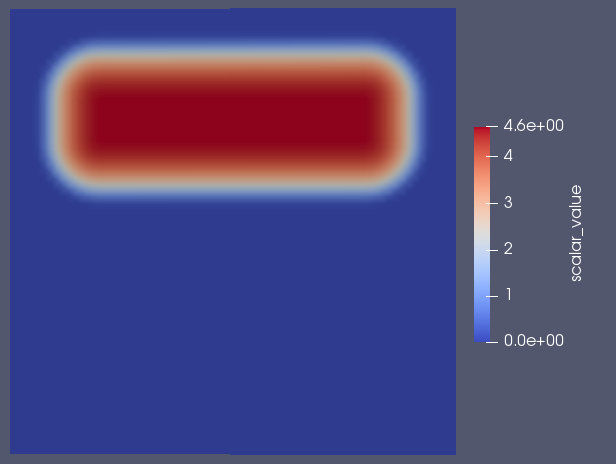
\includegraphics[width=0.55\textwidth]{anfangsbedingung.png} 
\end{figure}
Der Maximalwert ist dabei so gewählt, dass die Gesamtmasse der Anfangsbedingung gerade den Wert $ 1 $ ergibt.\\
Uns interessiert nun folgende Fragestellung: \\
\textbf{Wie groß ist der erwartete Anteil der Masse, welcher nach Ablauf des betrachteten Zeitintervalls $ \mathbb{T} $ im Rechengebiet $ \mathcal{D} $ verbleibt?}\\

Wie bereits an früherer Stelle erklärt, berechnen wir hierzu ein stochastische Flussvektorfeld $ q : \Omega \times \overline{\mathcal{ D}} \to \R^2 $ als Lösung des zugehörigen Potentialströmungsproblems, wobei wir dabei den Permeabilitätstensor $ \kappa : \Omega \times \mathcal{D} \to \R_{\geq0} $ als lognormal verteiltes Zufallsfeld modellieren. Wir identifizieren dabei die Verteilung von $ \kappa $ mit der zugehörigen Kovarianzfunktion:
\[
 C(x,y) = \sigma^2 \exp(- \frac{\lVert x-y \rVert_2^s}{\lambda^s} ) .
\]
Dabei ist $ 0 < \sigma^2 < \infty $ die Varianz des zugrundeliegenden Gauß'schen Zufallsfeldes, durch $ \lambda = (\lambda_1,\lambda_2) \in \R^2 $ werden die Korrelationslängen in die verschiedenen Koordinatenrichtungen gegeben und $ s \in (1,2) $ ist ein Glättungsparameter. \\
Wir können auch den das lognormal verteilte Zufallsfeld und das daraus resultierende stochastische Flussvektorfeld $ q $ exemplarisch für ein $ \omega \in \Omega $ grafisch darstellen. Bei der Visualisierung des Flussvektorfeldes nutzen wir dabei sogenannte 'Streamlines'. Im Wesentlichen nutzt man dabei einen Zeitintegrator, wie etwa ein Runge Kutta Verfahren, und integriert mit deren Hilfe an verschiedenen Ausgangspunkten entlang des Vektorfeldes.

\begin{figure}[H]
	\centering
	\captionabove{Visualisierung der stochastischen Modellierung}
	\subfigure[Streamlines des entstehenden Flussvektorfeldes]{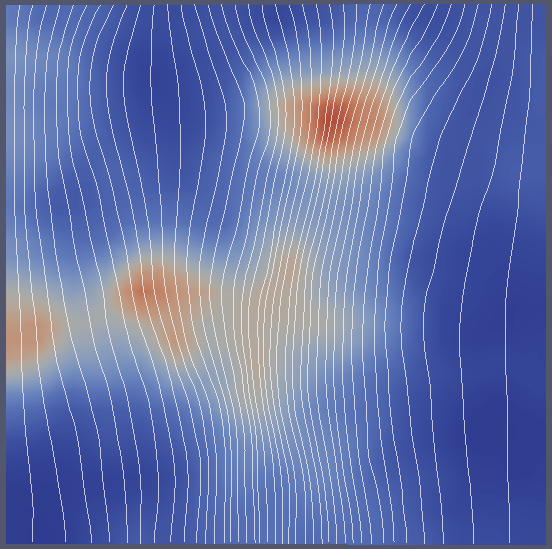
\includegraphics[width=0.423\textwidth]{flussvektorfeld.png}}
	\subfigure[lognormal verteiltes Zufallsfeld mit obigen Parametern]{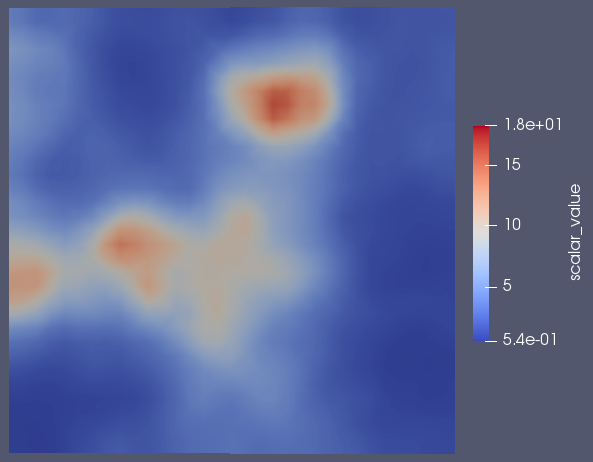
\includegraphics[width=0.54\textwidth]{perm.png}}
	
\end{figure}

Weiter setzen wir
\begin{itemize}
	\item $\Gamma_{\text{D}} = \{ x = (x_1,x_2) \in \overline{\mathcal{D}} : x_2 = 0 \} $
	\item $ \Gamma_{\text{N}} = \partial \mathcal{D} \setminus \Gamma_{\text{D}} $
	\item $ g_N = \begin{cases}
						\begin{array}{llll}
						    &0 &, &\text{falls } x \in \{ x \in \Gamma_{\text{N}} : x_1 \in \{ 0,1 \}  \} \\
						    &1 &,& \text{sonst}
						\end{array}
				  \end{cases} $
	\item $ u_D \equiv 0 \text{ auf } \Gamma_{\text{D}} $
	
\end{itemize}

Als Zerlegung von $ \mathcal{D} $ wählen wir gleichartige Quadrate. Um auf dem geringsten Level ein Mindestmaß an Auflösung zu gewährleisten wählen wir auf Level $ l_0 $ eine Zerlegung in $ 256 = 16^2 $ Quadrate. Dies entspricht einer Ortsdiskretisierungsschrittweite von $ h_0 = \frac{1}{16} = 0.0625 $. Wie bereits im Theorieteil angemerkt, wählen wir von $ h_0 $ ausgehend die uniforme Familie von Zerlegungen $ \{\mathcal{T}_h \}_{h \in \mathcal{H}} $ mit $ \mathcal{H} = \{ h_0 , h_1 \coloneqq \frac{h_0}{2},h_2 \coloneqq \frac{h_1}{2} = \frac{h_0}{4}, \dots \} $. Auf Level $ l_1 $ betrachten wir also $ 1024 = 32^2 $ und auf Level $ l_k $ dementsprechend $ 2^{2(k+4)} $ Quadrate. 
In M++ entspricht Level $ l_0 $ bei der gewählten Diskretisierung 'UnitSquare' gerade Level $ 4 $. Die Zerlegungen auf $ l_0 = 4, l_1 = 5 $ und $ l_2 = 6 $ lassen sich folgendermaßen darstellen:
\begin{figure}[H]
	\centering
	\captionabove{Zerlegung des Gebietes $ \mathcal{D} $ in Finite Elemente}
	\subfigure[$l_0$ (256 Zellen)]{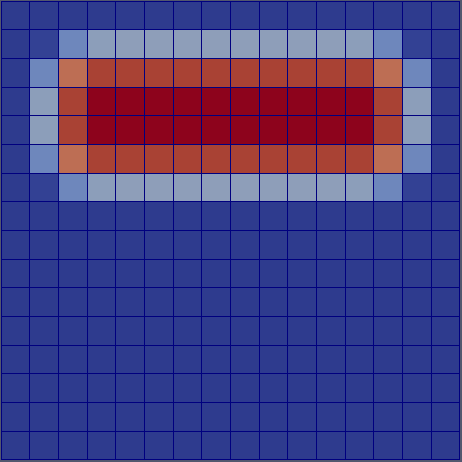
\includegraphics[width=0.3\textwidth]{zerlegung4.png}}
	\subfigure[$l_1$ (1024 Zellen)]{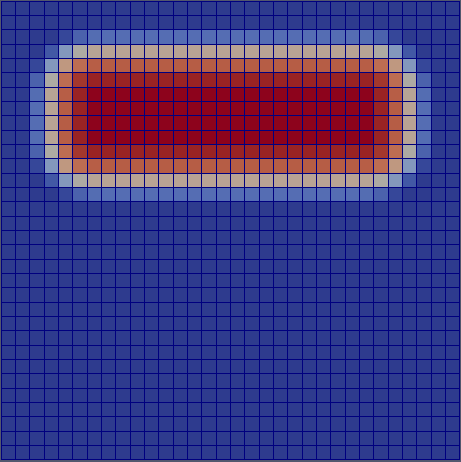
\includegraphics[width=0.3\textwidth]{zerlegung5.png}}
	\subfigure[$l_2$ (4096 Zellen)]{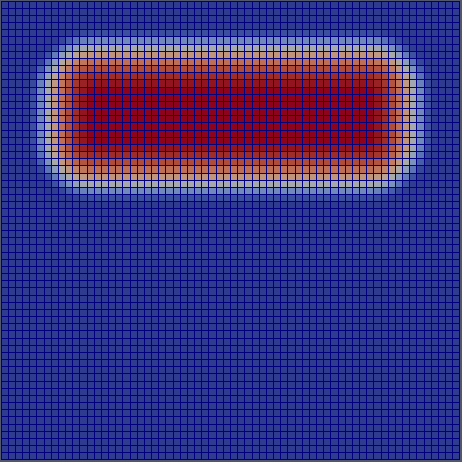
\includegraphics[width=0.3\textwidth]{zerlegung6.png}}
\end{figure}
Die Schrittweite für die Diskretisierung in der Zeit setzen wir auf $ \Delta t = \frac{h}{8} $. Diese Wahl ist besonders hinsichtlich der Stabilität des Verfahrens wichtig. Bei zu kleinen Zeitschrittweiten treten Oszillationen in der Lösung auf. Obige Wahl hat sich für unser Problem als hinreichend erwiesen.
Entsprechend unserer Fragestellung können wir nun das betrachtete Zielfunktional formulieren:
\[
Q(\omega) = J(\rho(\omega)) \coloneqq \int_{\mathcal{D}} \rho(\omega,x,T) \dx = \int_{\mathcal{D}} \rho(\omega,x,1) \dx
\]
Wir suchen gemäß unserer Fragestellung also gerade nach $ \mathbb{E}[Q] $.
\begin{Bemerkung2}\label{wahlfunk}
	Die Wahl $ T=1 $ ist an dieser Stelle gerade so getroffen, dass das der Fragestellung entsprechende Zielfunktional in gewisser Weise interessant ist. 
	Genauer ist $ T $ so gewählt, dass die im Algorithmus auftretende Varianz $ \mathbb{V}[Y_l] $ 'groß' ausfällt. Ist $ T $ nämlich zu groß gewählt befindet sich für fast alle $ \omega \in \Omega $ kaum noch Masse im Gebiet und die erwartete Endmasse ist $ \mathbb{E}[Q] = 0 $, während für sehr kleine $ T $ Masse zum Zeitpunkt $ T $ für fast alle $ \omega \in \Omega $ mit der Anfangsmasse übereinstimmt und somit $ \mathbb{E}[Q] = 1$. Für $ T = 1 $ erhalten wir für verschiedene $ \omega \in \Omega $ recht unterschiedliche Ergebnisse, da die Masse je nach Beschaffenheit des Flussvektorfeldes schneller oder langsamer durch das Gebiet transportiert wird. 
\end{Bemerkung2}

\subsection{Ergebnisse}


